\documentclass[11pt,a4paper]{article}
\usepackage[margin=18mm,top=22mm,bottom=20mm]{geometry}
\usepackage{fontspec}\setmainfont{Latin Modern Roman}
\usepackage{amsmath,amssymb,tikz,graphicx,fancyhdr,array,needspace}
\setlength{\headheight}{14pt}
\usetikzlibrary{arrows.meta}
\pagestyle{fancy}\fancyhf{}\renewcommand{\headrulewidth}{0.4pt}
\fancyhead[L]{\textbf{M-07}}\fancyhead[C]{\itshape Fizika (OliyFizika.uz mock test)}\fancyhead[R]{\textbf{Mock №7}}
\fancyfoot[C]{\thepage}
\setlength{\parindent}{0pt}\setlength{\parskip}{3pt}
\newcommand{\opt}[2]{\hspace*{4mm}#1)\ #2\par}
\newcommand{\blank}{\rule{5cm}{0.4pt}}
\begin{document}

\begin{center}{\Large\textbf{FIZIKA}}\end{center}
\noindent\begin{minipage}{\linewidth}
\textbf{1.}\ 10 m çuqurlikdagi odam tanasining bir santimetr kvadrat yuzasi suvning qanday bosim kuçi seziladi (N)? $\rho$=1000 kg/m$^{3}$. g=10 N/kg.\par\smallskip
\opt{A}{15}
\opt{B}{10}
\opt{C}{100}
\opt{D}{20}
\end{minipage}\vspace{9pt}\par
\noindent\begin{minipage}{\linewidth}
\textbf{2.}\ 80 kg massali odam köldan suzib ötiş uçun sol yasamoqçi. Agar solning qalinligi 20 cm bölsa, uning yuzasi (m$^{2}$) kamida qança bölişi kerak? Sol tayyorlanadigan yoğoçning ziçligi 600 kg/m$^{3}$, $\rho_{suv}$=1000 kg/m$^{3}$\par\smallskip
\opt{A}{1}
\opt{B}{1,4}
\opt{C}{0,8}
\opt{D}{1,2}
\end{minipage}\vspace{9pt}\par
\noindent\begin{minipage}{\linewidth}
\textbf{3.}\ Ikkita vertikal devor orasida yoruğlik manbai birinçi devordan 2 m masofa joylaşgan. Agar birinçi devorning yoritilganligi ikkinçi devorning yoritilganligidan 4 marta katta bölsa, devorlar orasidagi masofani toping (m).\par\smallskip
\opt{A}{4}
\opt{B}{6}
\opt{C}{3}
\opt{D}{8}
\end{minipage}\vspace{9pt}\par
\noindent\begin{minipage}{\linewidth}
\textbf{4.}\ Massasi 8 kg, hajmi 10 l bölgan tarvuz suvga tuşib ketsa, hajmining qança qismi suvga botadi?\par\smallskip
\opt{A}{0,6}
\opt{B}{0,5}
\opt{C}{0,8}
\opt{D}{0,25}
\end{minipage}\vspace{9pt}\par
\noindent\begin{minipage}{\linewidth}
\textbf{5.}\ Jism gorizontal sirtda tinç turibdi. Uni joyidan qözğatiş uçun kerak böladigan eng kiçik kuç 6 N. Jismga gorizontal yönalişda 5 N taşqi kuç qöyilsa, unga tezlaniş beruvçi (natijaviy) kuç (N) qanday böladi?\par\smallskip
\opt{A}{0}
\opt{B}{5}
\opt{C}{6}
\opt{D}{$-$1}
\end{minipage}\vspace{9pt}\par
\noindent\begin{minipage}{\linewidth}
\textbf{6.}\ Oq yoruğlik nuri difraksion panjaraga tik tuşmoqda. Bunda qaysi monoxromatik nur eng kam oğadi?\par\smallskip
\opt{A}{qizil}
\opt{B}{sariq}
\opt{C}{yaşil}
\opt{D}{binafşa}
\end{minipage}\vspace{9pt}\par
\noindent\begin{minipage}{\linewidth}
\textbf{7.}\ Matematik mayatnik arqonining uzunligi $\ell_{0}$ bölganda tebraniş davri T$_{0}$ ga teng. Uning uzunligi 20 cm ga ortganda tebraniş davri 3T$_{0}$ ga teng böldi. Mayatnik arqonining dastlabki uzunligini (cm) aniqlang.\par\smallskip
\opt{A}{20,0}
\opt{B}{2,5}
\opt{C}{22,5}
\opt{D}{17,5}
\end{minipage}\vspace{9pt}\par
\noindent\begin{minipage}{\linewidth}
\textbf{8.}\ Jism sinus qonuniga böysungan holda tebranmoqda. Tebraniş boşidan hisoblaganda qanday eng qisqa vaqtdan keyin jism impulsi 2 marta kamayadi? Jismning tebraniş davri T ga teng.\par\smallskip
\opt{A}{T/12}
\opt{B}{T/8}
\opt{C}{T/3}
\opt{D}{T/6}
\end{minipage}\vspace{9pt}\par
\noindent\begin{minipage}{\linewidth}
\textbf{9.}\ Ikki sterjen berilgan, mos ravişda ularning uzunliklari $l_1$ va $l_2$, çiziqli ziçliklari $\rho_1$ va $\rho_2$. Sterjenlarni rasmda körsatilganidek birlaştirsak, hosil bölgan sterjenda oğirlik kuçlari birinçi sterjenning taşqi uçiga nisbatan qanday kuç momenti hosil qiladi?\par\smallskip
\noindent\hspace*{4mm}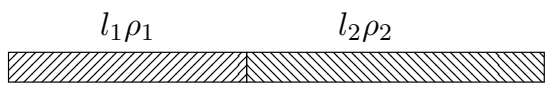
\includegraphics[width=0.6\linewidth,height=5.2cm,keepaspectratio]{../dtm-variantlari/rasmlar/8000273-04.png}\par\smallskip
\opt{A}{$\dfrac{g}{2}(\rho_1l_1^2+\rho_2l_2^2+2\rho_2l_1l_2)$}
\opt{B}{$g(\rho_1l_1^2+\rho_2l_2^2+2\rho_2l_1l_2)$}
\opt{C}{$\dfrac{g}{2}(l_1^2\rho_1+l_2^2\rho_2+l_1l_2\rho_2)$}
\opt{D}{$\dfrac{g}{2}(l_1^2\rho_1+l_2^3\rho_2+2l_1l_2\rho_2)$}
\end{minipage}\vspace{9pt}\par
\noindent\begin{minipage}{\linewidth}
\textbf{10.}\ Bir jinsli $M$ massali sterjen prujina va ip bilan rasmda körsatilganidek muvozanatga keltirilgan. Agar prujinaning bikrligi $k=1200$ N/m bölib 2 cm ga çözilgan bölsa, $M$ massani (kg) aniqlang. $g=10\ \mathrm{m/s^2}$\par\smallskip
\noindent\hspace*{4mm}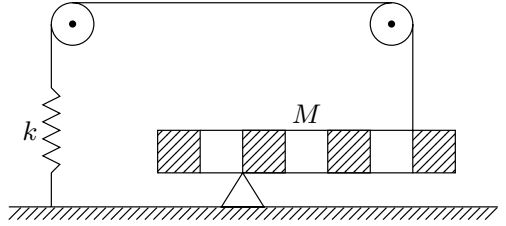
\includegraphics[width=0.6\linewidth,height=5.2cm,keepaspectratio]{../dtm-variantlari/rasmlar/1921920-21.png}\par\smallskip
\opt{A}{12,8}
\opt{B}{3,2}
\opt{C}{6,4}
\opt{D}{1,6}
\end{minipage}\vspace{9pt}\par
\noindent\begin{minipage}{\linewidth}
\textbf{11.}\ Ideal gazning içki energiyasi 144 kJ ga ortişi uçun gazga izoxorik ravişda qança issiqlik miqdori (kJ) berilişi kerak?\par\smallskip
\opt{A}{240}
\opt{B}{144}
\opt{C}{360}
\opt{D}{288}
\end{minipage}\vspace{9pt}\par
\noindent\begin{minipage}{\linewidth}
\textbf{12.}\ 44 g karbonat angidriddagi molekulalar soniga..... deb ataladi.\par\smallskip
\opt{A}{atom massa}
\opt{B}{konsentratsiya}
\opt{C}{molyar massa}
\opt{D}{Avogadro soni}
\end{minipage}\vspace{9pt}\par
\noindent\begin{minipage}{\linewidth}
\textbf{13.}\ Kapillar simobga tuşurilgan, simobning sirt taranglik koeffitsiyenti 0,51 N/m, ziçligi $13600\ \mathrm{kg/m^3}$. Simob kapillarni höllamagani uçun kapillar içidagi simob sathi atrofdagi sathdan 5 mm pastroq. Kapillarning içki radiusi (mm) qanday? $g=10\ \mathrm{m/s^2}$\par\smallskip
\opt{A}{0,19}
\opt{B}{1,5}
\opt{C}{0,37}
\opt{D}{0,75}
\end{minipage}\vspace{9pt}\par
\noindent\begin{minipage}{\linewidth}
\textbf{14.}\ Ballondagi kislorod gazining temperaturasini aniqlang (0 C). Taşqi atmosfera bosimi 1 atm=105 Pa ga teng. Kislorodning molyar massasi 32 g/mol.\par\smallskip
\noindent\hspace*{4mm}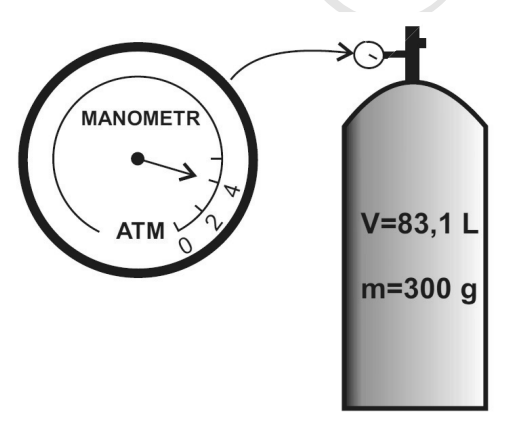
\includegraphics[width=0.6\linewidth,height=5.2cm,keepaspectratio]{../dtm-variantlari/rasmlar/T21-14.png}\par\smallskip
\opt{A}{140}
\opt{B}{147}
\opt{C}{232}
\opt{D}{260}
\end{minipage}\vspace{9pt}\par
\noindent\begin{minipage}{\linewidth}
\textbf{15.}\ Ikki idişda molekulalari soni teng bölgan bir xil temperaturadagi bir xil gazlar mavjud. Molekulalarning kvadratik tezligi mos ravişda: birinçi idişda 100 m/s ga, ikkinçisida esa 700 m/s ga teng. Agar idişlar özaro ulansa, molekulalar qanday qiymatdagi kvadratik tezlikka erişadi (m/s)?\par\smallskip
\opt{A}{400}
\opt{B}{500}
\opt{C}{600}
\opt{D}{350}
\end{minipage}\vspace{9pt}\par
\noindent\begin{minipage}{\linewidth}
\textbf{16.}\ 10 A tokka ulangan sterjen gorizontal holatda ikkita bir xil prujinaga osib qöyildi. Agar sterjen perpendikulyar magnit maydonda joylaşgan bölsa, prujinalarning çözilişini toping (cm). Sterjen uzunligi 20 cm. g=10 m/s$^{2}$.\par\smallskip
\noindent\hspace*{4mm}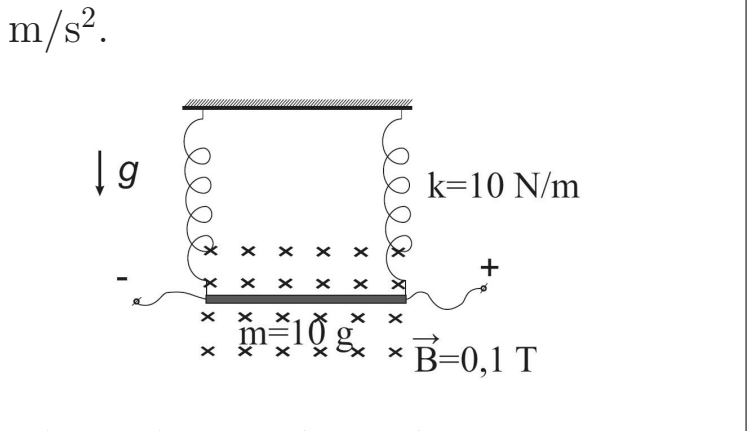
\includegraphics[width=0.6\linewidth,height=5.2cm,keepaspectratio]{../dtm-variantlari/rasmlar/T04-24.png}\par\smallskip
\opt{A}{3}
\opt{B}{1,5}
\opt{C}{2}
\opt{D}{0,5}
\end{minipage}\vspace{9pt}\par
\noindent\begin{minipage}{\linewidth}
\textbf{17.}\ Doimiy tok manbai içidagi çet kuçlar 6 C zaryadni elektrostatik kuçlarga qarşi yönalişda köçirişda 300 J iş bajardi. Tok manbaining EYK ini toping (V).\par\smallskip
\opt{A}{0,02}
\opt{B}{25}
\opt{C}{50}
\opt{D}{450}
\end{minipage}\vspace{9pt}\par
\noindent\begin{minipage}{\linewidth}
\textbf{18.}\ Nuqtaviy zaryad maydon kuçlanganligi zaryaddan 3,5 cm masofadagi nuqtada 150 V/m bölib, zaryad tomonga yönalgan. Şu nuqtadagi maydon potensiali (V) nimaga teng?\par\smallskip
\opt{A}{5,25}
\opt{B}{$-$3,75}
\opt{C}{$-$5,25}
\opt{D}{3,75}
\end{minipage}\vspace{9pt}\par
\noindent\begin{minipage}{\linewidth}
\textbf{19.}\ Dastlab çözilmagan, bikrligi k=62 N/m bölgan prujinaga m=62 g yuk osib qöyib yuborilganda A amplitudali garmonik tebranişlar yuzaga keldi. Prujina maksimal çözilganda yukning balandligini h=0 deb hisoblab, yukning potensial energiyasi maksimal bölgan paytda uning tezlanişi qanday böladi (m/s$^{2}$)?\par\smallskip
\opt{A}{9,8}
\opt{B}{5,4}
\opt{C}{4,9}
\opt{D}{0}
\end{minipage}\vspace{9pt}\par
\noindent\begin{minipage}{\linewidth}
\textbf{20.}\ $M$ va $N$ nuqtalar orqali ötuvçi ikki parallel, çeksiz uzun ötkazgiçlardan tok oqmoqda. $M$ ötkazgiçdagi tok kuçi $I$, $N$ ötkazgiçdagi 2$I$. Agar $M$ ötkazgiçdagi tokning $C$ nuqtada hosil qiladigan magnit induksiyasi $B$ bölsa, $C$ nuqtadagi umumiy magnit induksiya moduli nimaga teng? (qöşni nuqtalar orasidagi masofalar teng)\par\smallskip
\noindent\hspace*{4mm}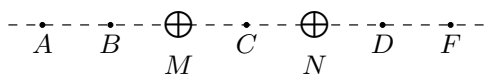
\includegraphics[width=0.6\linewidth,height=5.2cm,keepaspectratio]{../dtm-variantlari/rasmlar/8000897-13.png}\par\smallskip
\opt{A}{7$B$/3}
\opt{B}{3$B$/5}
\opt{C}{5$B$/3}
\opt{D}{$B$}
\end{minipage}\vspace{9pt}\par
\noindent\begin{minipage}{\linewidth}
\textbf{21.}\ Radiusi 1 m bölgan metall şar dielektik singdiruvçanligi 2 bölgan suyuqlikka botirilgan. Agar şar zaryadi 2 $\mu$C bölsa, uning energiyasini toping (mJ).\par\smallskip
\opt{A}{27}
\opt{B}{8}
\opt{C}{18}
\opt{D}{9}
\end{minipage}\vspace{9pt}\par
\noindent\begin{minipage}{\linewidth}
\textbf{22.}\ Induksiyasi $B$ bölgan magnit maydonda $m$ massali proton $v$ tezlik bilan aylanma harakatlanmoqda. Uning aylaniş radiusi qaysi formula bilan ifodalanadi?\par\smallskip
\opt{A}{$\dfrac{mv^2}{eB}$}
\opt{B}{$\dfrac{mv}{B}$}
\opt{C}{$\dfrac{mv}{eB}$}
\opt{D}{$\dfrac{2mv}{eB}$}
\end{minipage}\vspace{9pt}\par
\noindent\begin{minipage}{\linewidth}
\textbf{23.}\ Elektrolitlarda dissotsiatsiya darajasi (koeffitsiyenti) nimalarga boğliq?\par\smallskip
\opt{A}{temperaturaga}
\opt{B}{temperaturaga va eritmaning dielektrik singdiruvçanligiga}
\opt{C}{erituvçining dielektrik singdiruvçanligiga}
\opt{D}{erituvçining miqdoriga}
\end{minipage}\vspace{9pt}\par
\noindent\begin{minipage}{\linewidth}
\textbf{24.}\ Zaryadlangan kondensator qoplamalarini bir-biridan uzoqlaştirişda taşqi kuçlarning bajargan işi.....\par\smallskip
\opt{A}{nolga teng}
\opt{B}{manfiy}
\opt{C}{musbat}
\opt{D}{TJY}
\end{minipage}\vspace{9pt}\par
\noindent\begin{minipage}{\linewidth}
\textbf{25.}\ Induksiyasi 0,03 T bölgan bir jinsli magnit maydonga tik holatda 40 cm uzunlikdagi tokli ötkazgiç kiritildi. Undan 0,5 A tok ötkazilganda hosil böladigan amper kuçini (mN) aniqlang.\par\smallskip
\opt{A}{2}
\opt{B}{3}
\opt{C}{6}
\opt{D}{9}
\end{minipage}\vspace{9pt}\par
\noindent\begin{minipage}{\linewidth}
\textbf{26.}\ Balandligi 4 m bölgan xona şiftining markaziga lampa osilgan. Lampaning poldan balandligi 2 m. Agar polda xona markazida diametri 20 cm bölgan közgu yotgan bölsa, közgudan qaytgan nurlar şiftda qanday diametrli yoruğ doira hosil qiladi (cm)?\par\smallskip
\opt{A}{60}
\opt{B}{40}
\opt{C}{30}
\opt{D}{15}
\end{minipage}\vspace{9pt}\par
\noindent\begin{minipage}{\linewidth}
\textbf{27.}\ Davri 2,3 $\mu$m bölgan difraksion panjaraga tölqin uzunligi 0,6 $\mu$m bölgan tölqin tik tuşmoqda. Ekranda hosil bölgan maksimumlar sonini aniqlang.\par\smallskip
\opt{A}{6}
\opt{B}{3}
\opt{C}{7}
\opt{D}{4}
\end{minipage}\vspace{9pt}\par
\noindent\begin{minipage}{\linewidth}
\textbf{28.}\ Yerdan Oygaça bölgan masofa örtaça 384400 km ni taşkil etadi. Yerda fokus masofasi 50 cm bölgan linza yordamida Oyning haqiqiy tasviri hosil qilinmoqda. Bunda Oyning tasviri linzadan qanday masofada hosil böladi (cm)?\par\smallskip
\opt{A}{$\approx$75}
\opt{B}{$\approx$100}
\opt{C}{$\approx$25}
\opt{D}{$\approx$50}
\end{minipage}\vspace{9pt}\par
\noindent\begin{minipage}{\linewidth}
\textbf{29.}\ Tezligi 0,1$c$ bölgan zarraning töliq energiyasi $E$ ga teng. Zarraning tezligi uç marta ortsa, töliq energiyasi qanday böladi? $c$ - yoruğlik tezligi.\par\smallskip
\opt{A}{$9E$}
\opt{B}{$\sqrt{1{,}15}E$}
\opt{C}{$\sqrt{1{,}06}E$}
\opt{D}{$\sqrt{1{,}09}E$}
\end{minipage}\vspace{9pt}\par
\noindent\begin{minipage}{\linewidth}
\textbf{30.}\ Har bir atomga bittadan ötkazuvçanlik elektroni töğri keladi deb hisoblab, tok kuçi 50 A bölganda elektronlarning kesimi 25 mm$^{2}$ bölgan mis simdagi batartib harakatlaniş tezligini toping (mm/s). $\rho$=8900 kg/m$^{3}$, Ar (Cu)=64 u., NA =6$\cdot10^{23}$ mol$-$1.\par\smallskip
\opt{A}{1,5}
\opt{B}{0,15}
\opt{C}{15}
\opt{D}{0,015}
\end{minipage}\vspace{9pt}\par
\noindent\begin{minipage}{\linewidth}
\textbf{31.}\ Quyidagi parçalaniş reaksiyasidagi noma’lum $X$ zarrani aniqlang. ${}^{236}_{92}U \Rightarrow {}^{142}_{56}Ba + {}^{91}_{36}Kr + 3X$\par\smallskip
\opt{A}{${}^1_0n$}
\opt{B}{${}^4_2He$}
\opt{C}{${}^2_1H$}
\opt{D}{${}^1_1H$}
\end{minipage}\vspace{9pt}\par
\noindent\begin{minipage}{\linewidth}
\textbf{32.}\ Detalni defektoskop yordamida ultratovuşli tekşiruvdan ötkazganda detal sirtidan 10 cm çuqurligida kovak borligi aniqlandi. Agar ultratovuş signalining nuqsondan akslaniş (signalning borib keliş vaqti) vaqti 50 $\mu$s ga teng bölsa, tovuşning detal içida tarqaliş tezligini toping (m/s).\par\smallskip
\opt{A}{5000}
\opt{B}{8000}
\opt{C}{3000}
\opt{D}{4000}
\end{minipage}\vspace{9pt}\par
\newpage\noindent\textbf{33–35-test topshiriqlariga mos keluvchi javoblarni (A–F) javob variantlaridan tanlang.}\par\smallskip
Rasmda elektr zanjir tasvirlangan. Batareyaning ichki qarshiligi nolga teng, ampermetrlar ideal.\par\medskip
\begin{center}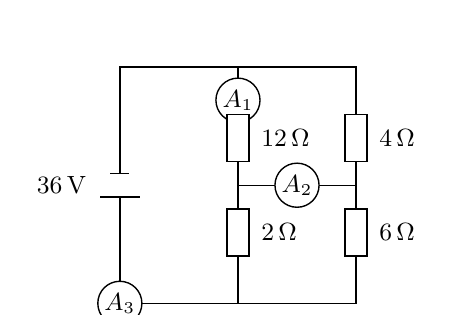
\begin{tikzpicture}[line width=0.5pt]
\draw (0,0)--(0,1.35); \draw (0,1.65)--(0,3)--(3,3)--(3,2.4); \draw (-0.25,1.35)--(0.25,1.35); \draw (-0.12,1.65)--(0.12,1.65);
\node[left] at (-0.3,1.5) {\small $36\,\mathrm{V}$};
\draw (1.5,3)--(1.5,2.72); \draw (1.5,2.44)--(1.5,2.4);
\draw (1.5,1.8)--(1.5,1.2); \draw (1.5,0.6)--(1.5,0)--(0.28,0); \draw (-0.28,0)--(0,0);
\draw (3,1.8)--(3,1.2); \draw (3,0.6)--(3,0)--(1.5,0);
\draw (1.5,1.5)--(1.97,1.5); \draw (2.53,1.5)--(3,1.5);
\draw[fill=white] (1.5,2.58) circle (0.28); \node at (1.5,2.58) {\small $A_1$};
\draw[fill=white] (1.3599999999999999,1.8) rectangle (1.6400000000000001,2.4); \node[right] at (1.67,2.1) {\small $12\,\Omega$};
\draw[fill=white] (1.3599999999999999,0.6000000000000001) rectangle (1.6400000000000001,1.2); \node[right] at (1.67,0.9) {\small $2\,\Omega$};
\draw[fill=white] (2.86,1.8) rectangle (3.14,2.4); \node[right] at (3.17,2.1) {\small $4\,\Omega$};
\draw[fill=white] (2.86,0.6000000000000001) rectangle (3.14,1.2); \node[right] at (3.17,0.9) {\small $6\,\Omega$};
\draw[fill=white] (2.25,1.5) circle (0.28); \node at (2.25,1.5) {\small $A_2$};
\draw[fill=white] (0.0,0.0) circle (0.28); \node at (0.0,0.0) {\small $A_3$};
\end{tikzpicture}\end{center}
\noindent\fbox{\begin{minipage}{0.64\linewidth}\vspace{4pt}\textbf{33.}\ $A_1$ ampermetrning körsatişini (A) aniqlang.\\[6pt]\textbf{34.}\ $A_2$ ampermetrning körsatişini (A) aniqlang.\\[6pt]\textbf{35.}\ $A_3$ ampermetrning körsatişini (A) aniqlang.\vspace{4pt}\end{minipage}\vrule\hspace{6pt}\begin{minipage}{0.28\linewidth}\vspace{4pt}A)\ 4\\B)\ 8\\C)\ 2\\D)\ 5\\E)\ 1\\F)\ 6\vspace{4pt}\end{minipage}}\par\vspace{14pt}
\Needspace{9\baselineskip}
\noindent\textbf{36.}\ Qirrasining uzunligi 2 cm bölgan kub şaklidagi 4 ta muz bölagi asosining yuzasi 60 cm$^2$ bölgan, 91,2 g suv quyilgan silindrik idişda taşlandi. $\rho_{muz}=900$ kg/m$^3$.\par\smallskip
\medskip\noindent\textbf{a)\ Muzlar erib ketgandan söng suyuqlikning idiş tubiga beradigan bosimini (Pa) toping.}\par
\noindent\textit{Javob}: a)\ \blank\par
\medskip\noindent\textbf{b)\ Muzlar erib ketgandan söng suyuqlikning idiş tubiga beradigan bosim kuçini (N) hisoblang.}\par
\noindent\textit{Javob}: b)\ \blank\par
\medskip\noindent\textbf{Diqqat!} Javoblaringizni javoblar varaqasiga köçirib yozing.\par\vspace{10pt}
\Needspace{9\baselineskip}
\noindent\textbf{37.}\ Silindrik idişga teng massali suv va kerosin quyildi. Suyuqliklar ustunining umumiy balandligi 18 cm ga teng. $\rho_{kerosin}=800$ kg/m$^3$.\par\smallskip
\medskip\noindent\textbf{a)\ Suv ustunining balandligini (cm) aniqlang.}\par
\noindent\textit{Javob}: a)\ \blank\par
\medskip\noindent\textbf{b)\ Idiş tubidan 10 cm balandlikdagi nuqtada suyuqliklarning hosil qilgan umumiy bosimini (Pa) toping.}\par
\noindent\textit{Javob}: b)\ \blank\par
\medskip\noindent\textbf{Diqqat!} Javoblaringizni javoblar varaqasiga köçirib yozing.\par\vspace{10pt}
\Needspace{9\baselineskip}
\noindent\textbf{38.}\ Uzunligi 48 m, qiyalik burçagi $37^\circ$ bölgan silliq qiya tekislik tepasidan 12 kg massali jism sirpanib tuşdi. $\sin37^\circ=0,6$, $\cos37^\circ=0,8$.\par\smallskip
\medskip\noindent\textbf{a)\ Jismning qiya tekislik etagidagi tezligini (m/s) toping.}\par
\noindent\textit{Javob}: a)\ \blank\par
\medskip\noindent\textbf{b)\ Bu jarayonda oğirlik kuçining bajargan işini (J) toping.}\par
\noindent\textit{Javob}: b)\ \blank\par
\medskip\noindent\textbf{Diqqat!} Javoblaringizni javoblar varaqasiga köçirib yozing.\par\vspace{10pt}
\Needspace{9\baselineskip}
\noindent\textbf{39.}\ Bir atomli ideal gazga 125 J issiqlik berib, hajmi izobarik ravişda 6 marta oşirildi.\par\smallskip
\medskip\noindent\textbf{a)\ Bunda gazning absolyut temperaturasi qanday özgaradi?}\par
\noindent\textit{Javob}: a)\ \blank\par
\medskip\noindent\textbf{b)\ Gazning bajargan işini (J) aniqlang.}\par
\noindent\textit{Javob}: b)\ \blank\par
\medskip\noindent\textbf{Diqqat!} Javoblaringizni javoblar varaqasiga köçirib yozing.\par\vspace{10pt}
\Needspace{9\baselineskip}
\noindent\textbf{40.}\ Issiqlik siğimi 350 J/K bölgan idişda 6 $^\circ$C temperaturali 5 $\ell$ suv bor. Idişga $-4\,^\circ$C temperaturali 0,8 kg muz taşlandi. $c_{suv}=4200$ J/(kg$\cdot$K), $c_{muz}=2100$ J/(kg$\cdot$K), $\lambda_{muz}=330$ kJ/kg.\par\smallskip
\medskip\noindent\textbf{a)\ Natijaviy temperaturani ($^\circ$C) toping.}\par
\noindent\textit{Javob}: a)\ \blank\par
\medskip\noindent\textbf{b)\ Muzning olgan issiqlik miqdorini (kJ) aniqlang.}\par
\noindent\textit{Javob}: b)\ \blank\par
\medskip\noindent\textbf{Diqqat!} Javoblaringizni javoblar varaqasiga köçirib yozing.\par\vspace{10pt}
\Needspace{9\baselineskip}
\noindent\textbf{41.}\ Proton induksiyasi $B$ bölgan magnit maydonga tik uçib kirdi va $r$ radiusli aylana böylab harakatlana boşladi. $m$ — zarraning massasi, $e$ — elementar zaryad.\par\smallskip
\medskip\noindent\textbf{a)\ Uning markazga intilma tezlanişini aniqlang.}\par
\noindent\textit{Javob}: a)\ \blank\par
\medskip\noindent\textbf{b)\ Aylaniş çastotasini aniqlang.}\par
\noindent\textit{Javob}: b)\ \blank\par
\medskip\noindent\textbf{Diqqat!} Javoblaringizni javoblar varaqasiga köçirib yozing.\par\vspace{10pt}
\Needspace{9\baselineskip}
\noindent\textbf{42.}\ Maydon kuçlanganligi $E$ bölgan bir jinsli elektr maydonda harakatlanayotgan alfa-zarra ($q=2e$) $l$ masofaga köçib, $A$ nuqtadan $B$ nuqtaga yetib bordi (rasmda $AD\perp \vec E$).\par\smallskip
\begin{center}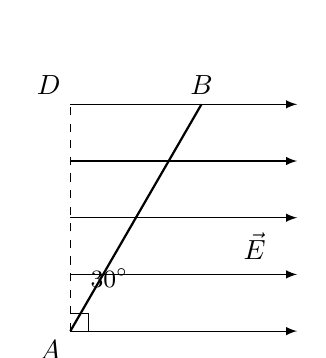
\begin{tikzpicture}[scale=0.9]\foreach \y in {0,0.8,1.6,2.4,3.2}{\draw[-latex] (0,\y)--(3.2,\y);}\draw (0.25,0)--(0.25,0.25)--(0,0.25);\draw[dashed] (0,0)--(0,3.2);\draw[thick] (0,0)--(1.85,3.2);\node[below left] at (0,0) {$A$};\node[above left] at (0,3.2) {$D$};\node[above] at (1.85,3.2) {$B$};\node at (2.6,1.2) {$\vec E$};\node at (0.55,0.75) {\small $30^\circ$};\end{tikzpicture}\end{center}
\medskip\noindent\textbf{a)\ Zarraning kinetik energiyasi qançaga özgarganini aniqlang.}\par
\noindent\textit{Javob}: a)\ \blank\par
\medskip\noindent\textbf{b)\ Zarra $ABDA$ yopiq yöl böylab köçirilganda elektr kuçlar bajaradigan işni aniqlang.}\par
\noindent\textit{Javob}: b)\ \blank\par
\medskip\noindent\textbf{Diqqat!} Javoblaringizni javoblar varaqasiga köçirib yozing.\par\vspace{10pt}
\Needspace{9\baselineskip}
\noindent\textbf{43.}\ Suvdagi nurning intensivligi 90 W/m$^2$ ga teng. $c=3\cdot10^8$ m/s.\par\smallskip
\medskip\noindent\textbf{a)\ Nurdagi elektromagnit maydon energiyasining ziçligini (J/m$^3$) aniqlang.}\par
\noindent\textit{Javob}: a)\ \blank\par
\medskip\noindent\textbf{b)\ Nur suvdagi közgudan tik akslansa, közguga beradigan bosimini (Pa) aniqlang.}\par
\noindent\textit{Javob}: b)\ \blank\par
\medskip\noindent\textbf{Diqqat!} Javoblaringizni javoblar varaqasiga köçirib yozing.\par\vspace{10pt}
\Needspace{9\baselineskip}
\noindent\textbf{44.}\ Oyning diametri $3,5\cdot10^{6}$ m ga, Yer bilan Oyn orasidagi masofa $3,8\cdot10^{8}$ m ga teng. Fokus masofasi 0,3 m bölgan Yerdagi linza ekranda Oynning haqiqiy tasvirini hosil qilmoqda.\par\smallskip
\medskip\noindent\textbf{a)\ Tasvir bilan linza orasidagi masofani (mm) toping.}\par
\noindent\textit{Javob}: a)\ \blank\par
\medskip\noindent\textbf{b)\ Oyn tasvirining diametrini (mm) toping.}\par
\noindent\textit{Javob}: b)\ \blank\par
\medskip\noindent\textbf{Diqqat!} Javoblaringizni javoblar varaqasiga köçirib yozing.\par\vspace{10pt}
\Needspace{9\baselineskip}
\noindent\textbf{45.}\ Ğalayonlangan vodorod atomining ionlaşiş energiyasi 3,4 eV ga teng.\par\smallskip
\medskip\noindent\textbf{a)\ Atom fotonni yutib impuls momentini $3\hbar$ ga oşirsa, uning ionlaniş energiyasi (eV) nimaga teng bölişini aniqlang.}\par
\noindent\textit{Javob}: a)\ \blank\par
\medskip\noindent\textbf{b)\ Atom fotonni yutib impuls momentini $3\hbar$ ga oşirsa, undagi elektronning tezligi neça marta özgarişini aniqlang.}\par
\noindent\textit{Javob}: b)\ \blank\par
\medskip\noindent\textbf{Diqqat!} Javoblaringizni javoblar varaqasiga köçirib yozing.\par\vspace{10pt}
\end{document}